\documentclass[11pt,a4paper]{article}
\usepackage[utf8]{inputenc}
\usepackage[T1]{fontenc}
\usepackage{lmodern}
\usepackage[spanish,es-noshorthands,es-tabla]{babel}
\usepackage[a4paper,margin=2.4cm,headheight=14pt]{geometry}
\usepackage{amsmath,amssymb}
\usepackage{graphicx}
\usepackage{booktabs}
\usepackage{multirow}
\usepackage{xcolor}
\usepackage{caption}
\usepackage{fancyhdr}
\usepackage{listings}
\usepackage[most]{tcolorbox}
\usepackage[hidelinks]{hyperref}

\graphicspath{{figures/}}
\emergencystretch=3em
\captionsetup{font=small,labelfont=bf}
\definecolor{verde}{RGB}{0,110,40}
\newtcolorbox{comando}[1]{colback=gray!6,colframe=verde,fonttitle=\bfseries\small,title={#1},boxrule=0.6pt,left=4pt,right=4pt,top=2pt,bottom=2pt}
\lstset{basicstyle=\ttfamily\footnotesize,columns=fullflexible,keepspaces=true,frame=none,
  literate={á}{{\'a}}1 {é}{{\'e}}1 {í}{{\'i}}1 {ó}{{\'o}}1 {ú}{{\'u}}1 {ñ}{{\~n}}1}
\pagestyle{fancy}\fancyhf{}
\lhead{\small\itshape Práctica 2 -- RL tabular sin modelo}\rhead{\small J.C. J.G. A.G.}\cfoot{\thepage}

\newcommand{\UR}{{\nearrow}}
\newcommand{\DR}{{\searrow}}
\newcommand{\qe}{q_\varepsilon}

\begin{document}
\begin{titlepage}\centering
{\large\bfseries Aprendizaje por Refuerzo\par}\vspace{2mm}
Grado en Ingeniería Matemática e Inteligencia Artificial (IMAT) -- 4º A\\ Universidad Pontificia Comillas, ICAI\par
\vspace{2.2cm}\rule{\textwidth}{0.6pt}\par\vspace{4mm}
{\LARGE Práctica 2:\par}\vspace{2mm}{\Large\bfseries RL tabular sin modelo:\\ SARSA y Q-learning\par}
\vspace{4mm}\rule{\textwidth}{0.6pt}\par\vspace{2cm}
{\large\bfseries Informe de laboratorio\par}\vspace{2cm}
Jorge Carnicero\\ Jorge González\\ Andrés Gil\par\vspace{1cm}
{\bfseries Fecha de entrega:\\ octubre de 2026\par}
\vfill
\begin{minipage}{0.92\textwidth}\small\tableofcontents\end{minipage}
\end{titlepage}

%=====================================================================
\section{Introducción y metodología}

En la Práctica~1 resolvimos \emph{Jump To The Goal} con programación dinámica, usando el modelo $p(s',r\mid s,a)$. Ahora el agente no lo conoce: aprende solo de las transiciones $(S_t,A_t,R_{t+1},S_{t+1})$ que genera. Implementamos los dos métodos de diferencias temporales (TD) tabulares, SARSA y Q-learning, y analizamos qué estiman, cuánta experiencia necesitan y por qué difieren.

\textbf{Configuración basal.} Entorno determinista, $\gamma=0.9$, $r_s=-1$, $r_{obs}=-5$, $r_{goal}=+5$, $\varepsilon=0.2$, $\alpha=0.1$ y $Q_0=0$ (valores por defecto de \texttt{main.py}), $20\,000$ episodios ($\approx 80\,000$ pasos) y estado inicial uniforme en $s_{init}=\{s_0,s_4,s_8,s_{12}\}$.

\textbf{Metodología.} (i) Validamos la implementación con 32 comprobaciones automáticas del script \texttt{validate\_\allowbreak algorithms.py}: reglas de actualización con azar guionizado, ausencia de \emph{bootstrapping} en transiciones terminales, desempate de \texttt{argmax}, y que con $\varepsilon=0$ ambos algoritmos generan exactamente la misma tabla $Q$. (ii) Un ejecutor instrumentado llama a las funciones de episodio originales, reproduce bit a bit \texttt{main.py} y registra $Q$ completa, visitas $N(s,a)$, retornos y una evaluación greedy ($\varepsilon=0$) desde los cuatro estados iniciales cada 20 episodios. (iii) Cada configuración se repite con 10 semillas (20 en la basal), las mismas para ambos algoritmos, lo que permite comparaciones pareadas; damos medias, percentiles e intervalos bootstrap al 95\,\%. (iv) Las referencias teóricas se calculan con el modelo $P$, que nunca se entrega a los agentes. En total, 400 entrenamientos.

Distinguimos \emph{pasos} (transiciones globales), \emph{episodios} y \emph{visitas} a un par. El \emph{retorno} es la suma sin descuento de un episodio, como lo registra \texttt{entrenamiento.py}.

\begin{comando}{Reproducción (desde \texttt{lab2/experiments})}
\ttfamily\small python validate\_algorithms.py\\ python run\_experiments.py\\ python analyze\_results.py
\end{comando}

%=====================================================================
\section{Trabajo previo: valores óptimos \texorpdfstring{$q_*$}{q*}}

Con el modelo determinista, $q_*$ cumple la ecuación de optimalidad de Bellman
\begin{equation}
q_*(s,a)=r(s,a)+\gamma\max_{a'}q_*(s',a'),\qquad q_*(T,\cdot)=0 .
\label{eq:bellman}
\end{equation}
El agente siempre avanza una columna (o cae una fila en la última), así que el grafo de transiciones es acíclico y $q_*$ se obtiene hacia atrás: $q_*(s_7,\cdot)=5$, $q_*(s_3,\cdot)=-1+0.9\cdot 5=3.5$, $q_*(s_6,\UR)=-1+0.9\cdot3.5=2.15$, $q_*(s_{13},\UR)=-1+0.9\,q_*(s_{11},\UR)=2.15$ y $q_*(s_{13},\DR)=-1+0.9\max_{a}q_*(s_{18},a)=-5.5$. La Tabla~\ref{tab:qstar} recoge los 40 valores, que coinciden con $v_*=\max_a q_*$ de Policy y Value Iteration de la Práctica~1 en los 21 estados.

\begin{table}[!htbp]\centering\small
\begin{tabular}{crrcl}
\toprule
Estado & $q_*(s,\nearrow)$ & $q_*(s,\searrow)$ & $\mathcal{A}_*(s)$ & Observación \\
\midrule
$s_{0}$ & $-$5.0000 & 0.9350 & $\searrow$ &  \\
$s_{1}$ & $-$5.0000 & $-$5.0000 & $\nearrow,\searrow$ & sin ruta al objetivo, misma transición \\
$s_{2}$ & $-$5.0000 & 3.5000 & $\searrow$ & inalcanzable \\
$s_{3}$ & 3.5000 & 3.5000 & $\nearrow,\searrow$ & misma transición \\
$s_{4}$ & $-$5.5000 & $-$0.1585 & $\searrow$ &  \\
$s_{5}$ & $-$5.0000 & 2.1500 & $\searrow$ &  \\
$s_{6}$ & 2.1500 & 5.0000 & $\searrow$ &  \\
$s_{7}$ & 5.0000 & 5.0000 & $\nearrow,\searrow$ & misma transición \\
$s_{8}$ & 0.9350 & $-$5.0000 & $\nearrow$ &  \\
$s_{9}$ & $-$5.0000 & 0.9350 & $\searrow$ &  \\
$s_{10}$ & 3.5000 & 3.5000 & $\nearrow,\searrow$ & empate, rutas distintas \\
$s_{11}$ & 3.5000 & $-$5.9500 & $\nearrow$ &  \\
$s_{12}$ & $-$0.1585 & $-$5.0000 & $\nearrow$ &  \\
$s_{13}$ & 2.1500 & $-$5.5000 & $\nearrow$ &  \\
$s_{14}$ & 5.0000 & $-$5.5000 & $\nearrow$ &  \\
$s_{15}$ & $-$5.5000 & $-$5.5000 & $\nearrow,\searrow$ & sin ruta al objetivo, misma transición \\
$s_{16}$ & $-$5.0000 & $-$5.0000 & $\nearrow,\searrow$ & inalcanzable, sin ruta al objetivo, misma transición \\
$s_{17}$ & 3.5000 & $-$5.0000 & $\nearrow$ & inalcanzable \\
$s_{18}$ & $-$5.9500 & $-$5.0000 & $\searrow$ & sin ruta al objetivo \\
$s_{19}$ & $-$5.0000 & $-$5.0000 & $\nearrow,\searrow$ & sin ruta al objetivo, misma transición \\
\bottomrule
\end{tabular}

\caption{Valores óptimos $q_*(s,a)$ ($\gamma=0.9$, $r_s=-1$, $r_{obs}=-5$, $r_{goal}=+5$) y acciones óptimas $\mathcal{A}_*(s)$.}
\label{tab:qstar}
\end{table}

\begin{figure}[!htbp]\centering
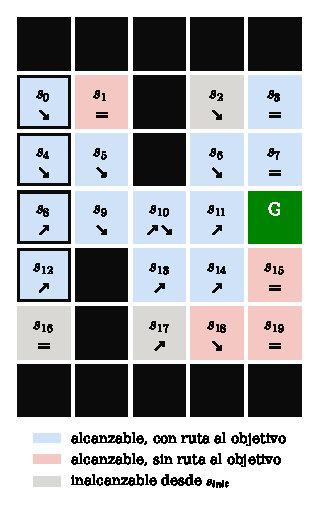
\includegraphics[width=0.36\textwidth]{fig_map.pdf}
\caption{Estructura del entorno: acción óptima ($=$: ambas acciones producen la misma transición) y estados iniciales (recuadro).}
\label{fig:map}
\end{figure}

Del modelo extraemos cuatro propiedades que condicionan el aprendizaje (Figura~\ref{fig:map}):
\begin{itemize}\itemsep0pt
\item \textbf{Inalcanzables:} $s_2$, $s_{16}$ y $s_{17}$ solo tienen obstáculos como predecesores ($s_{16}$ está en la primera columna pero fuera de $s_{init}$). Un método sin modelo no puede aprender sus $Q$, que se quedarán en $Q_0$. No es un fallo del algoritmo: su convergencia exige visitar cada par.
\item \textbf{Sin ruta al objetivo:} desde $s_1$, $s_{15}$, $s_{18}$ y $s_{19}$ solo se puede chocar; lo óptimo es minimizar la pérdida ($s_{18}$ choca ya, $-5$, en lugar de $s_{18}\to s_{15}\to s_{19}\to T$, $-5.95$).
\item \textbf{Empates:} en $s_1$, $s_3$, $s_7$, $s_{15}$ y $s_{19}$ ambas acciones producen la misma transición; en $s_{10}$, en cambio, dos rutas distintas ($s_6$ y $s_{14}$) valen $3.5$.
\item \textbf{Riesgo exploratorio:} $q_*$ supone que después se actuará de forma óptima. Un error desde $s_{14}$ lleva a un choque seguro ($q_*(s_{14},\DR)=-5.5$), mientras que desde $s_6$ solo alarga el camino ($q_*(s_6,\UR)=2.15$). Esta asimetría explicará la principal diferencia entre los algoritmos.
\end{itemize}

%=====================================================================
\section{SARSA}
\subsection{Fundamentos e implementación}

SARSA es un método TD(0) de control: tras cada transición actualiza
\begin{equation}
Q(S,A)\leftarrow Q(S,A)+\alpha\big[R+\gamma Q(S',A')-Q(S,A)\big],
\end{equation}
donde $A'$ es la acción que se ejecutará realmente en $S'$, elegida con la misma política $\varepsilon$-greedy (\emph{on-policy}). Si $S'$ es terminal el target es solo $R$. El target sustituye el retorno completo por una estimación (\emph{bootstrapping}), por lo que el $+5$ se propaga hacia atrás un estado por visita.

\begin{lstlisting}
next_action = epsilon_greedy(Q, next_state, epsilon, rng)          # A' que se ejecutará
Q[state,action] += alpha*(reward + gamma*Q[next_state,next_action] - Q[state,action])
Q[state,action] += alpha*(reward - Q[state,action])                # si S' es terminal
\end{lstlisting}

\textbf{Qué estima.} Con transiciones deterministas, el valor esperado del target dado $Q$ es
\begin{equation}
(T_\varepsilon Q)(s,a)=r+\gamma\Big[(1-\varepsilon)\max_{a'}Q(s',a')+\tfrac{\varepsilon}{2}\textstyle\sum_{a'}Q(s',a')\Big].
\label{eq:Teps}
\end{equation}
$T_\varepsilon$ es una contracción de módulo $\gamma$ con punto fijo único $\qe$, el valor de la mejor política $\varepsilon$-greedy. Con $\varepsilon$ constante, SARSA fluctúa alrededor de $\qe$, \emph{no} de $q_*$. Converge a $q_*$ con probabilidad 1 si la exploración es GLIE ($\varepsilon_k\to0$ visitando todos los pares infinitas veces) y $\alpha$ cumple Robbins--Monro ($\sum\alpha_k=\infty$, $\sum\alpha_k^2<\infty$) [3]. Con $\alpha$ constante y targets aleatorios, $Q$ no se detiene nunca: fluctuar es el comportamiento esperado, no un error.

\subsection{Convergencia en \texorpdfstring{$s_6$}{s6} y \texorpdfstring{$s_{13}$}{s13}}

\begin{figure}[!htbp]\centering
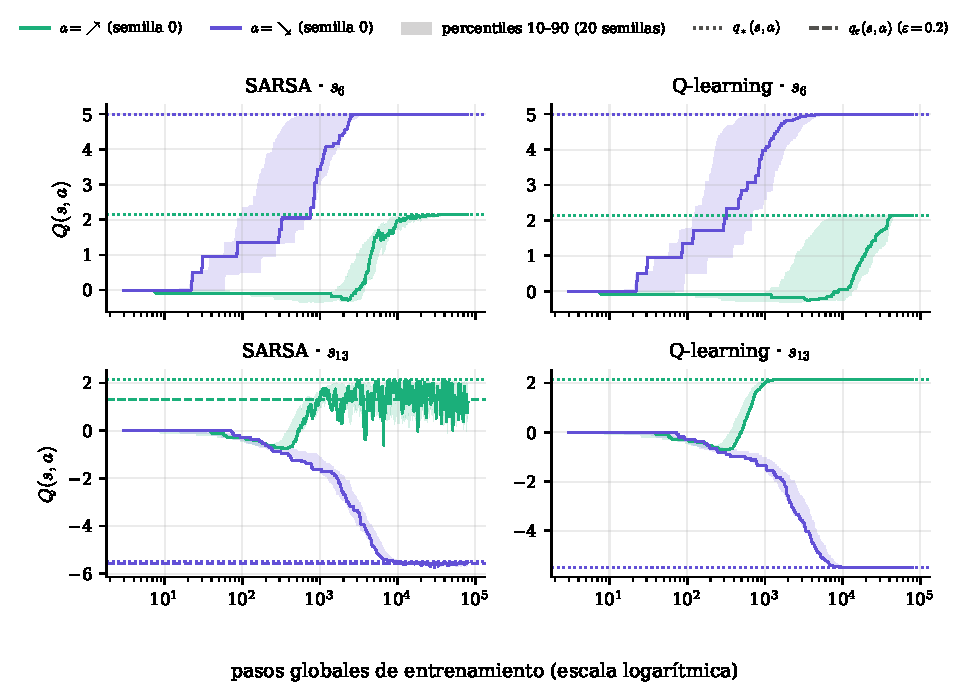
\includegraphics[width=\textwidth]{fig_q_s6_s13.pdf}
\caption{Evolución de $Q(s_6,\cdot)$ y $Q(s_{13},\cdot)$ frente a pasos globales (configuración basal).}
\label{fig:q}
\end{figure}

\textbf{Estado $s_6$} (Figura~\ref{fig:q}, izquierda). Ninguna acción depende de decisiones futuras: $\DR$ termina en el objetivo y $\UR$ recorre $s_3\to s_7\to T$, donde las dos acciones de $s_3$ y $s_7$ hacen lo mismo. Por ello $\qe(s_6,\cdot)=q_*(s_6,\cdot)=(2.15,\,5)$ y SARSA converge sin ruido.
\begin{itemize}\itemsep0pt
\item $Q(s_6,\DR)\leftarrow Q+\alpha(5-Q)$: el error decae como $5(1-\alpha)^n$ (en nuestras notas escribimos $\gamma$ en lugar de $\alpha$) y entra en la banda $\pm0.1$ tras $\ln(0.02)/\ln(0.9)\approx38$ visitas (mediana medida: 40; 1\,873 pasos).
\item $Q(s_6,\UR)$ empieza \emph{negativa} (mínimo medio $-0.31$): su target $-1+\gamma Q(s_3,\cdot)$ usa $Q(s_3)\approx0$, así que el $-1$ llega antes que el $+5$. Se vuelve positiva cuando el valor se propaga $s_7\to s_3\to s_6$ y alcanza $2.15$ tarde (mediana 10\,372 pasos), porque al ser no greedy solo se elige al explorar: 693 visitas frente a 6\,160 de $\DR$. Converge más despacio porque recibe menos muestras, no porque sea más difícil.
\end{itemize}

\textbf{Estado $s_{13}$, acción $\DR$.} Lleva a $s_{18}$, desde donde solo se puede chocar. Con probabilidad $0.9$ el agente elige después $\DR$ (target $-1+0.9(-5)=-5.5$) y con $0.1$ elige $\UR$ ($-1+0.9(-5.95)=-6.355$), luego $\qe(s_{13},\DR)=-5.586$. Medimos $-5.583$ (media temporal del último 25\,\%, 20 semillas). En nuestras notas afirmábamos que convergía a $-5.5$: converge a $-5.59$, y las caídas que observábamos son esas muestras exploratorias.

\textbf{Estado $s_{13}$, acción $\UR$.} Lleva a $s_{11}$, una bifurcación: $\UR$ conduce al objetivo ($Q(s_{11},\UR)=3.5$) y $\DR$ a un choque seguro ($Q(s_{11},\DR)=-5.95$). El target vale $2.15$ con probabilidad $0.9$ y $-6.355$ con $0.1$:
\begin{equation}
\qe(s_{13},\UR)=-1+0.9\,(0.9\cdot3.5+0.1\cdot(-5.95))=1.2995<q_*(s_{13},\UR)=2.15 .
\end{equation}
La media medida es $1.302$, lo que confirma la predicción. Fases: hasta $\sim\!500$ pasos ambas $Q$ son negativas (solo se han propagado los $-1$); entre $500$ y $3\,000$ pasos $Q(s_{13},\UR)$ sube a medida que $s_{11}$ aprende; después oscila alrededor de $1.30$. Cada punto de la curva es un valor instantáneo, no el esperado: una sola elección exploratoria en $s_{11}$ lo baja en $\alpha(Q+6.355)\approx0.77$, y la recuperación es geométrica.

\subsection{Influencia de los hiperparámetros}

\begin{figure}[!htbp]\centering
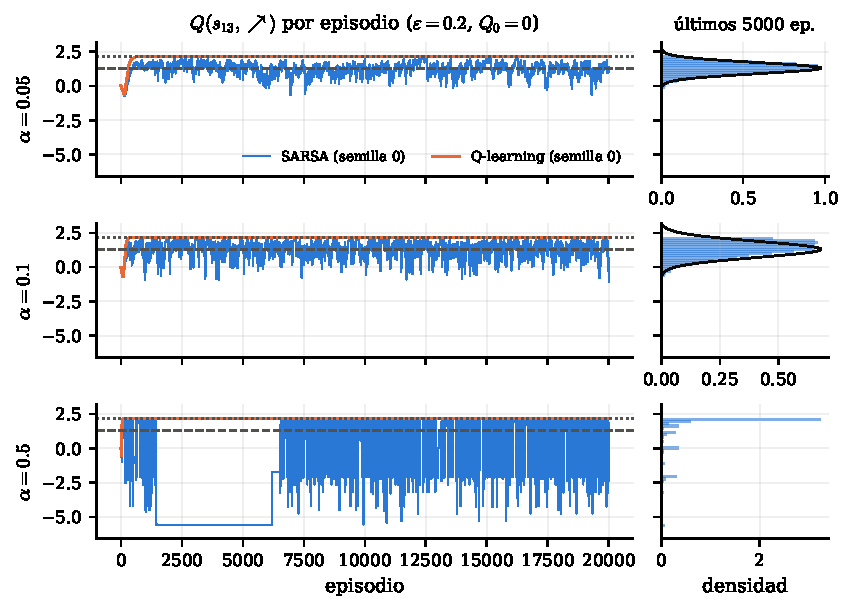
\includegraphics[width=\textwidth]{fig_alpha_s13.pdf}
\caption{$Q(s_{13},\UR)$ de SARSA y Q-learning para tres valores de $\alpha$. Derecha: distribución en los últimos 5\,000 episodios (10 semillas) y normal teórica $\mathcal N(\qe,\sigma^2)$ para $\alpha\le0.1$. Líneas: $q_*$ (puntos) y $\qe$ (trazos).}
\label{fig:alpha}
\end{figure}

\begin{table}[!htbp]\centering\small
\begin{tabular}{lcccccccc}
\toprule
 & \multicolumn{3}{c}{SARSA: $Q(s_{13},\nearrow)$} & QL & \multicolumn{2}{c}{Retorno greedy} & \multicolumn{2}{c}{Política estable (ep.)} \\
\cmidrule(lr){2-4}\cmidrule(lr){6-7}\cmidrule(lr){8-9}
$\alpha$ & $\sigma$ teórica & $\sigma$ emp. & media emp. & media & SARSA & QL & SARSA & QL \\
\midrule
0.01 & 0.18 & 0.17 & 1.33 & 2.15 & 1.50 & 1.50 & 17\,187 & 17\,602 \\
0.05 & 0.41 & 0.41 & 1.29 & 2.15 & 1.50 & 1.50 & 3\,436 & 3\,368 \\
0.1 & 0.59 & 0.58 & 1.31 & 2.15 & 1.50 & 1.50 & 1\,597 & 1\,414 \\
0.5 & 1.47 & 1.66 & 1.19 & 2.15 & 1.17 & 1.50 & 1/10 nunca & 202 \\
1.0 & 2.55 & 4.12 & $-$3.17 & 2.15 & $-$4.90 & 1.50 & 10/10 nunca & 75 \\
\bottomrule
\end{tabular}

\caption{Efecto de $\alpha$ (10 semillas). $\sigma$: desviación típica estacionaria de $Q(s_{13},\UR)$. Política estable: episodio desde el que la acción greedy es óptima en los 17 estados alcanzables.}
\label{tab:alpha}
\end{table}

\textbf{Tasa de aprendizaje.} Entre visitas a $(s_{13},\UR)$, las $Q$ de $s_{11}$ ya son constantes, así que $Q_{n+1}=(1-\alpha)Q_n+\alpha X_n$ es un proceso AR(1) con $X_n$ independientes de media $\qe$ y desviación $\sigma_X=\gamma\sqrt{0.1\cdot0.9}\,(3.5+5.95)=2.55$. Su media estacionaria es $\qe$ para cualquier $\alpha$ y su varianza, $\alpha\sigma_X^2/(2-\alpha)$. La Tabla~\ref{tab:alpha} lo confirma para $\alpha\le0.1$ ($\sigma$ teórica/empírica: $0.18/0.17$, $0.41/0.41$, $0.59/0.58$) con medias entre $1.29$ y $1.33$: $\alpha$ no cambia \emph{qué} estima SARSA, sino la velocidad y el ruido. Más velocidad cuesta más ruido: la política tarda 17\,187 episodios en estabilizarse con $\alpha=0.01$ y 1\,597 con $\alpha=0.1$.

Con $\alpha\ge0.5$ la aproximación falla porque el ruido realimenta la política. En la semilla~0 con $\alpha=0.5$ (Figura~\ref{fig:alpha}, segmento plano), dos exploraciones seguidas en $s_{11}$ hunden $Q(s_{13},\UR)$ por debajo de $Q(s_{13},\DR)$ en el episodio 1\,444. El error se propaga aguas arriba: en $s_9$, $s_4$ y $s_{12}$ chocar ($-5$) pasa a parecer mejor que continuar ($\approx-5.5$). $s_{13}$ apenas vuelve a visitarse y el error persiste unos 4\,800 episodios. El 11\,\% de las evaluaciones posteriores al episodio 1\,000 son subóptimas. Con $\alpha=1$, $Q$ es la última muestra: el choque tiene valor determinista $-5$ y continuar vale lo que dio la última muestra, a menudo contaminada por un error exploratorio aguas abajo. La política greedy acaba chocando desde los cuatro estados iniciales (retorno $-4.90$).

\textbf{Número de episodios.} Con $\alpha$ y $\varepsilon$ constantes, entrenar $N$ episodios es exactamente el prefijo de un entrenamiento más largo con la misma semilla (comprobado). El presupuesto no cambia la dinámica, solo dónde se detiene. Con 500 episodios ($\approx2\,000$ pasos) $Q(s_6,\DR)$ está prácticamente aprendida (mediana: 1\,873 pasos) y $Q(s_{13},\UR)$ ronda $\qe$. Con 2\,000, la política es óptima en los 17 estados (mediana: episodio 1\,509). Más allá de $\sim\!10\,000$, $Q$ ya no mejora: solo queda ruido estacionario. \emph{La política se estabiliza mucho antes que los valores}, y estos nunca se detienen.

\begin{figure}[!htbp]\centering
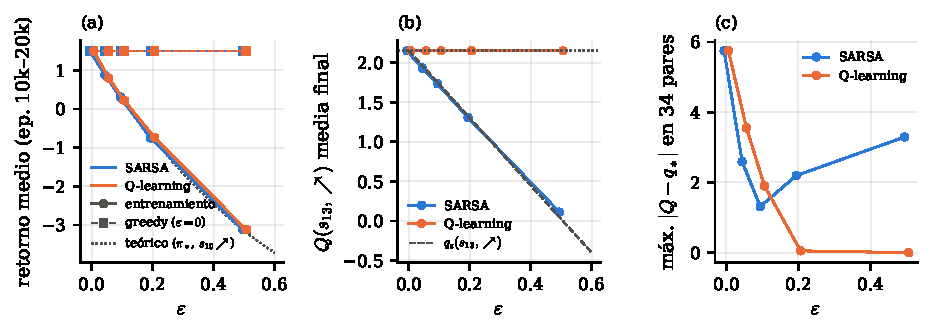
\includegraphics[width=\textwidth]{fig_epsilon.pdf}
\caption{Efecto de $\varepsilon$ (10 semillas, $\alpha=0.1$, $Q_0=0$). (a) Retorno de entrenamiento y greedy, con la predicción exacta para la política $\varepsilon$-greedy de $\pi_*$. (b) Media final de $Q(s_{13},\UR)$ y curva $\qe(s_{13},\UR)$. (c) Error máximo frente a $q_*$ en los pares alcanzables.}
\label{fig:eps}
\end{figure}

\textbf{Exploración.} $\varepsilon$ sí cambia el objetivo: $\qe(s_{13},\UR)=-1+0.9\,[(1-\tfrac{\varepsilon}{2})3.5-\tfrac{\varepsilon}{2}5.95]$ es lineal en $\varepsilon$, y las medias empíricas siguen esa recta (Figura~\ref{fig:eps}b). Más exploración aumenta el impacto de las decisiones arriesgadas: la tasa de éxito en entrenamiento cae del 92.6\,\% ($\varepsilon=0.05$) al 72.8\,\% ($0.2$) y al 42.5\,\% ($0.5$). El retorno coincide con el valor exacto de la conducta $\varepsilon$-greedy (Figura~\ref{fig:eps}a). La política greedy es óptima en todos los casos, por lo que la pérdida se debe a explorar, no a aprender mal.

\begin{figure}[!htbp]\centering
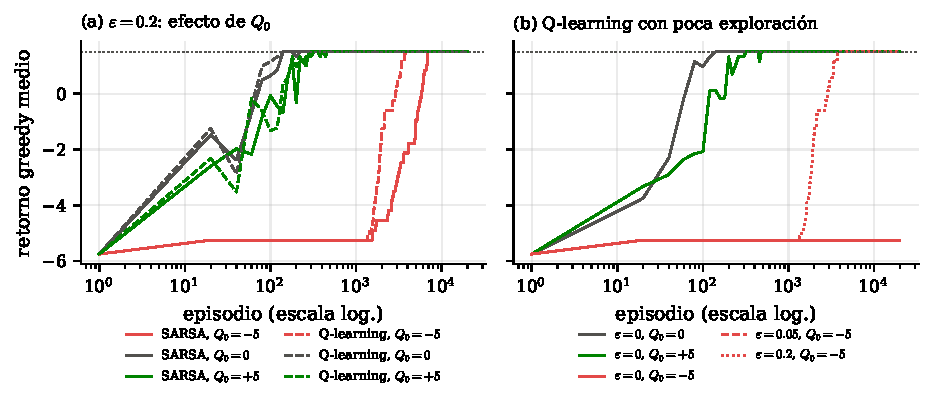
\includegraphics[width=\textwidth]{fig_qinit.pdf}
\caption{Retorno greedy medio desde $s_{init}$ (10 semillas). (a) Efecto de $Q_0$ con $\varepsilon=0.2$. (b) Q-learning con poca exploración (con $\varepsilon=0$ SARSA es idéntico).}
\label{fig:q0}
\end{figure}

\textbf{Inicialización.} $Q_0=0$ es optimista para 19 de los 34 pares alcanzables ($q_*<0$): una acción que acaba mal baja de 0 y la alternativa no probada pasa a ser greedy. Esto es exploración dirigida. Con $Q_0=-5$ (pesimista), chocar tiene target $-5=Q_0$ y no cambia nada, mientras que dar un paso tiene target $-1+0.9(-5)=-5.5<-5$. El agente prefiere chocar hasta que la exploración descubre el objetivo y el valor se propaga: la evaluación greedy tarda 5\,790 episodios en ser óptima (80 con $Q_0=0$; Figura~\ref{fig:q0}a). $Q_0=+5$ aprende igual de rápido y prueba más al principio (retorno $-1.58$ frente a $-1.43$ en 500 episodios). Además, los pares con $q_*=5$ ($s_6\DR$, $s_7$, $s_{14}\UR$) empiezan ya en su valor exacto. Tras suficientes visitas, $Q_0$ solo deja huella en los pares poco visitados, con un factor $(1-\alpha)^N$.

\textbf{Interacciones.} La combinación peligrosa es poca exploración con pesimismo: con $\varepsilon=0$ y $Q_0=-5$ el agente choca en todos los episodios, y con $\varepsilon=0.05$ el éxito es del 0.06\,\% tras 20\,000 episodios (Figura~\ref{fig:q0}b; SARSA se comporta igual), porque propagar el valor hasta $s_{init}$ exige varias exploraciones consecutivas. El optimismo puede sustituir a la exploración: con $\varepsilon=0$ y $Q_0=+5$ la política es óptima en 130 episodios. Con $\alpha$ y $\varepsilon$ altos ($0.5/0.5$), SARSA acumula ambos ruidos: retorno greedy final $0.38$ frente a $1.50$ con $\alpha=0.05$.

\textbf{Extensión GLIE.} Con $\varepsilon_k=0.2/(1+k/1000)$, que acaba en 0.0095, $Q(s_{13},\UR)$ alcanza $2.10\pm0.15$, muy cerca de $q_*=2.15$, como predice la teoría.

%=====================================================================
\section{Q-learning}
\subsection{Fundamentos}

Q-learning actualiza con el máximo del estado siguiente:
\begin{equation}
Q(S,A)\leftarrow Q(S,A)+\alpha\big[R+\gamma\max_{a'}Q(S',a')-Q(S,A)\big].
\end{equation}
Es \emph{off-policy}: la conducta es $\varepsilon$-greedy, pero el target evalúa la política greedy, la acción que se ejecute después no interviene. Su valor esperado es la ecuación de optimalidad~\eqref{eq:bellman} ($T_0$, una contracción con punto fijo $q_*$). Converge a $q_*$ con probabilidad 1 si todos los pares se visitan infinitas veces y $\alpha$ cumple Robbins--Monro [2]. En un entorno determinista el target no tiene ruido. Con $\alpha$ constante, una vez exactos los sucesores, $|Q_{n+1}-q_*|=(1-\alpha)|Q_n-q_*|$: converge sin fluctuaciones, pero solo en los pares visitados.

\subsection{Convergencia en \texorpdfstring{$s_6$}{s6} y \texorpdfstring{$s_{13}$}{s13}}

En $s_6$ (Figura~\ref{fig:q}, derecha) Q-learning y SARSA tienen el mismo target, porque no hay bifurcación aguas abajo. Por visita aprenden igual ($Q(s_6,\DR)$ entra en la banda tras 38 visitas). Sin embargo, en pasos tardan el doble (3\,759 frente a 1\,873 en $\DR$; 38\,939 frente a 10\,372 en $\UR$), porque durante los primeros $10\,000$ episodios su conducta pasa sobre todo por $s_{14}$ y no por $s_6$ (Sección~\ref{sec:comp}).

En $s_{13}$ el target de $\UR$ usa $\max_a Q(s_{11},a)=3.5$, aunque después la conducta explore $\DR$ en $s_{11}$. Por eso $Q(s_{13},\UR)\to2.15$ con desviación final $2\cdot10^{-13}$, frente a $0.58$ en SARSA, y $Q(s_{13},\DR)\to-5.5$. Las fases son las mismas que en SARSA (valores negativos, propagación, final), pero el final es un punto fijo exacto.

\begin{figure}[!htbp]\centering
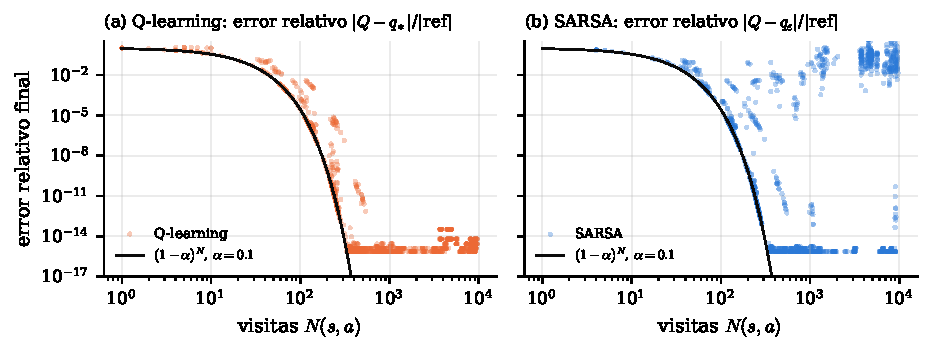
\includegraphics[width=\textwidth]{fig_visits_error.pdf}
\caption{Error relativo final frente a visitas, para todos los pares alcanzables ($\alpha=0.1$, $\varepsilon\in\{0.05,0.1,0.2,0.5\}$, 10 semillas). Referencia: $q_*$ para Q-learning, $\qe$ para SARSA.}
\label{fig:visits}
\end{figure}

La Figura~\ref{fig:visits}a muestra que el error de cada par sigue $(1-\alpha)^N$ hasta la precisión de máquina ($10^{-16}$). Los puntos desplazados a la derecha son pares cuyos sucesores convergieron más tarde. Esto explica los errores residuales: $Q(s_3,\UR)$, con 37 visitas en la semilla~0, vale $3.42$ (error $0.08\approx3.5\cdot0.9^{37}$). En SARSA (Figura~\ref{fig:visits}b), los pares con target determinista siguen la misma curva, pero los que tienen una bifurcación aguas abajo se estancan en un suelo de ruido entre $10^{-2}$ y $1$.

\subsection{Influencia de los hiperparámetros}

\textbf{$\alpha$.} Sin ruido en el target, un $\alpha$ mayor solo acelera: la política es óptima en los 17 estados tras 1\,414 episodios con $\alpha=0.1$, 202 con $0.5$ y 75 con $\alpha=1$ (Tabla~\ref{tab:alpha}). Con $\alpha=1$ cada actualización es un \emph{backup} de Bellman exacto, como una Value Iteration asíncrona sobre la experiencia. Es el comportamiento opuesto al de SARSA.

\textbf{$\varepsilon$.} No cambia el objetivo ($Q(s_{13},\UR)=2.15$ para todo $\varepsilon$, Figura~\ref{fig:eps}b), pero sí la \emph{cobertura}. Las acciones no greedy solo se aprenden explorando. Con $\varepsilon=0.05$, $Q(s_6,\UR)=0.08$ tras 20\,000 episodios (frente a $2.15$) y el error máximo es $3.56$; con $\varepsilon=0.5$ es $5\cdot10^{-11}$ (Figura~\ref{fig:eps}c). El coste de explorar recae en el retorno de entrenamiento, igual que en SARSA.

\textbf{$Q_0$ y $\varepsilon=0$.} $Q_0=-5$ retrasa el aprendizaje (2\,840 episodios hasta la política greedy óptima, Figura~\ref{fig:q0}a) y $Q_0=+5$ da el menor error final ($0.001$). Con $\varepsilon=0$ y $Q_0=+5$ el retorno greedy es óptimo, pero 3 pares no se visitan nunca y algunos estados fuera de la trayectoria conservan una acción incorrecta (error máximo $10.5$). Una política óptima \emph{sobre su trayectoria} no implica valores ni acciones correctos en todos los estados.

%=====================================================================
\section{Comparación entre SARSA y Q-learning}\label{sec:comp}

Respuestas a las preguntas del enunciado, que justificamos a continuación con los cuatro criterios. \emph{¿Misma política?} Sí: ambas son óptimas y solo pueden diferir en el empate de $s_{10}$. \emph{¿Mismos valores?} No: Q-learning converge a $q_*$ y SARSA a $\qe$. \emph{¿Mejor retorno en entrenamiento?} SARSA, en la fase intermedia (500--10\,000 episodios), porque evita la ruta en la que explorar es más caro. En evaluación greedy ambos son idénticos.

\begin{figure}[!htbp]\centering
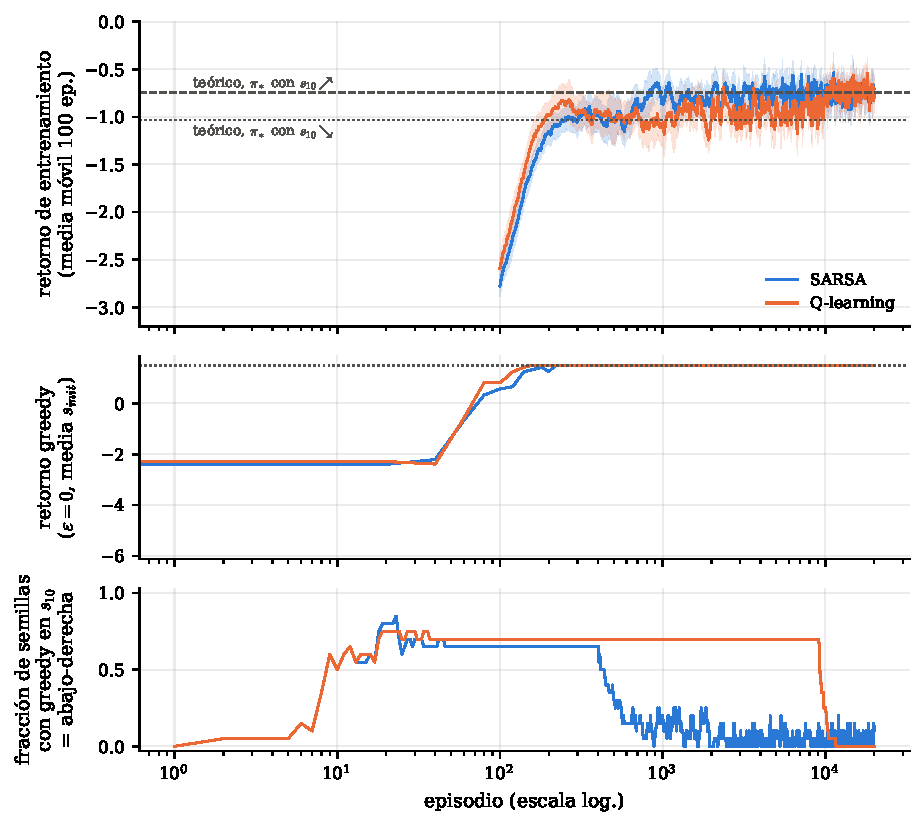
\includegraphics[width=\textwidth]{fig_returns.pdf}
\caption{Configuración basal, 20 semillas. Arriba: retorno de entrenamiento (media móvil de 100 episodios, IC 95\,\%) y valor exacto de la conducta $\varepsilon$-greedy de $\pi_*$ según la ruta elegida en $s_{10}$. Centro: retorno greedy. Abajo: fracción de semillas cuya acción greedy en $s_{10}$ es $\DR$.}
\label{fig:returns}
\end{figure}

\begin{table}[!htbp]\centering\footnotesize
\begin{tabular}{lccccccc}
\toprule
 & \multicolumn{2}{c}{Retorno medio} & & & & \multicolumn{2}{c}{greedy$(s_{10})=\searrow$} \\
\cmidrule(lr){2-3}\cmidrule(lr){7-8}
Episodios & SARSA & QL & Dif. [IC 95\,\%] & $p$ & SARSA mejor & SARSA & QL \\
\midrule
{}[0, 100) & $-$2.78 & $-$2.59 & $-$0.19 [$-$0.31, $-$0.07] & 0.008 & 5/20 & 61\,\% & 65\,\% \\
{}[100, 500) & $-$1.05 & $-$0.99 & $-$0.06 [$-$0.15, 0.02] & 0.157 & 6/20 & 60\,\% & 70\,\% \\
{}[500, 10\,000) & $-$0.76 & $-$0.94 & 0.18 [0.12, 0.24] & $<0.001$ & 15/20 & 6\,\% & 67\,\% \\
{}[10\,000, 20\,000) & $-$0.76 & $-$0.75 & $-$0.02 [$-$0.04, 0.00] & 0.130 & 7/20 & 4\,\% & 1\,\% \\
\bottomrule
\end{tabular}

\caption{Retorno de entrenamiento por fases (20 semillas pareadas). Dif.: SARSA $-$ QL con IC bootstrap al 95\,\%; $p$: test de permutación de signos.}
\label{tab:returns}
\end{table}

\textbf{A. Eficiencia muestral.} Con $\alpha\le0.1$ no hay diferencias relevantes (Figura~\ref{fig:eff}). Ambos alcanzan el retorno greedy óptimo desde $s_{init}$ hacia el episodio 80 ($\approx300$--$450$ pasos) y la acción óptima en los 17 estados hacia el 1\,500. La diferencia aparece con $\alpha$: Q-learning mejora de forma monótona hasta $\alpha=1$, porque su target es determinista, y SARSA empeora desde $\alpha=0.5$, porque el suyo es ruidoso. Para un mismo par con target determinista ambos necesitan las mismas visitas. Las diferencias en pasos se deben a cuántas veces visita cada conducta ese par (caso de $s_6$). En ambos, la política se estabiliza mucho antes que los valores.

\begin{figure}[!htbp]\centering
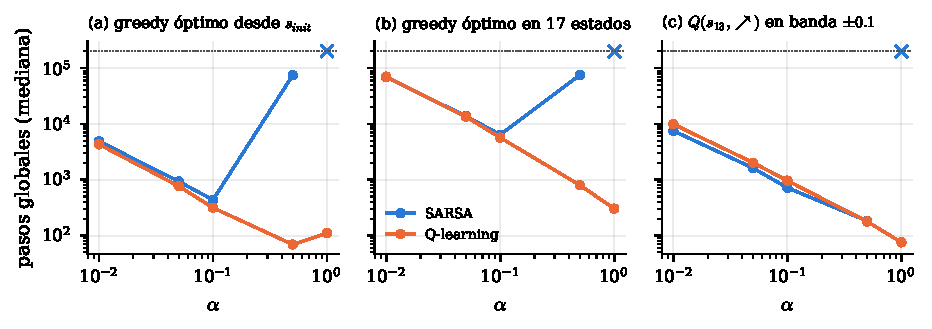
\includegraphics[width=\textwidth]{fig_efficiency.pdf}
\caption{Pasos globales (mediana de 10 semillas) hasta que, de forma estable, (a) la política greedy es óptima desde $s_{init}$ y (b) en los 17 estados alcanzables, y (c) hasta que $Q(s_{13},\UR)$ entra por primera vez en $\pm0.1$ de su referencia. ×: la mayoría de semillas no lo alcanza.}
\label{fig:eff}
\end{figure}

\textbf{B. Evolución del retorno} (Figura~\ref{fig:returns}, Tabla~\ref{tab:returns}). La evaluación greedy es idéntica: $1.5$ en ambos, el óptimo. En entrenamiento distinguimos tres fases.
\begin{itemize}\itemsep0pt
\item \emph{Inicial (0--100 episodios).} Ambos chocan con frecuencia (retorno $\approx-2.7$). Q-learning es algo mejor ($-0.19$, $p=0.008$), lo que es coherente con que el máximo propaga antes el valor del objetivo. La ventaja de su política greedy entre los episodios 20 y 200 no es significativa ($p=0.08$).
\item \emph{Intermedia (500--10\,000).} SARSA obtiene $0.18$ más por episodio (IC $[0.12,0.24]$, $p<0.001$, 15 de 20 semillas). La causa es $s_{10}$: la acción greedy de Q-learning es $\DR$ en el 67\,\% de los casos, la de SARSA en el 6\,\%. Explorando en $s_{14}$ se pierden 11 puntos (choque en lugar de $+5$), y en $s_6$ solo 2. El valor exacto de la conducta $\varepsilon$-greedy es $-0.741$ por $s_6$ frente a $-1.033$ por $s_{14}$, y $0.67\times0.29\approx0.20$ coincide con lo medido. SARSA \emph{ve} este riesgo, $\qe(s_{10},\UR)=3.24>\qe(s_{10},\DR)=2.56$; para Q-learning ambas valen $3.5$.
\item \emph{Final (10\,000--20\,000).} La diferencia desaparece ($p=0.13$), pero no porque Q-learning aprenda el riesgo.
\end{itemize}

\textbf{¿Por qué Q-learning elige $s_{14}$ y por qué deja de hacerlo?} Con $Q_0=0$, \texttt{argmax} desempata hacia $\UR$. En $s_{14}$, $\UR$ es la acción que llega al objetivo y $Q(s_{14},\UR)$ aprende el $+5$ enseguida; en $s_6$, $\UR$ es el rodeo. Al principio $\max Q(s_{14})>\max Q(s_6)$, así que $\DR$ domina en $s_{10}$. Al recibir más actualizaciones, queda más cerca de $3.5$ por debajo y se mantiene greedy. Es una preferencia que se autorrefuerza. Hacia el episodio 9\,300, tras unas 390 visitas, la acción no greedy alcanza \emph{exactamente} $3.5$ en doble precisión ($3.5\cdot0.9^n$ es menor que medio ulp para $n\approx354$), y \texttt{argmax} resuelve el empate exacto hacia $\UR$. Es un artefacto numérico, no aprendizaje. Con $\varepsilon=0.05$ ese empate no llega en 20\,000 episodios y la ventaja de SARSA persiste hasta el final ($+0.08$, $p=0.004$; predicción $0.9\times0.10$).

\textbf{C. Exploración frente a explotación.} SARSA incorpora en sus valores su propia exploración futura: estima la conducta que realmente ejecuta y prefiere rutas robustas a los errores. Q-learning aprende sobre la política greedy objetivo, ignora que la conducta explora y por eso alcanza $q_*$ incluso con $\varepsilon=0.5$, pero no distingue rutas igual de buenas sin exploración y distintas con ella. Las políticas difieren solo donde los $\arg\max$ de $\qe$ y $q_*$ difieren. Lo comprobamos para $\varepsilon\le0.5$ y $r_{obs}$ hasta $-50$: solo ocurre en $s_{10}$, que es un empate en $q_*$, así que ambas políticas finales son óptimas. Explorar demasiado poco puede bloquear el aprendizaje ($\varepsilon=0$, $Q_0=-5$); explorar demasiado hunde el retorno de entrenamiento ($-3.1$ con $\varepsilon=0.5$) y aleja a SARSA de $q_*$, aunque mejora la cobertura de Q-learning.

\textbf{D. Valores finales} (Tabla~\ref{tab:final}).
\begin{itemize}\itemsep0pt
\item \emph{Q-learning:} los 34 pares alcanzables convergen a $q_*$. El error máximo es $\le0.08$ y siempre aparece en pares con menos de 100 visitas ($s_3$ en 16 de 20 semillas).
\item \emph{SARSA:} converge a $\qe$ (por ejemplo, $-1.815$ frente a $-1.815$ en $s_4\DR$; $1.30$ en $s_{13}\UR$). Difiere de $q_*$ siempre que aguas abajo haya una bifurcación con consecuencias asimétricas: $s_0\DR$ $0.05$ frente a $0.94$, $s_4\DR$ $-1.81$ frente a $-0.16$. Los pares cuya trayectoria posterior es determinista ($s_6$, $s_{11}$, $s_{14}$, $s_{18}$, última columna) coinciden en ambos.
\item \emph{Inalcanzables:} $s_2$, $s_{16}$ y $s_{17}$ conservan $Q_0$ en los dos algoritmos. Es falta de experiencia, no un error de estimación.
\end{itemize}

\begin{table}[!htbp]\centering\scriptsize\setlength{\tabcolsep}{2.8pt}
\begin{tabular}{c rrrrr rrrrr}
\toprule
 & \multicolumn{5}{c}{$a=\nearrow$} & \multicolumn{5}{c}{$a=\searrow$} \\
\cmidrule(lr){2-6}\cmidrule(lr){7-11}
$s$ & $q_*$ & $q_\varepsilon$ & SARSA ($\sigma$) & QL & $N$ S/QL & $q_*$ & $q_\varepsilon$ & SARSA ($\sigma$) & QL & $N$ S/QL \\
\midrule
$s_{0}$ & $-$5.00 & $-$5.00 & $-$5.00 (0.00) & $-$5.00 & 498/504 & 0.94 & 0.05 & 0.05 (0.42) & 0.94 & 4498/4501 \\
$s_{1}$ & $-$5.00 & $-$5.00 & $-$5.00 (0.00) & $-$5.00 & 255/253 & $-$5.00 & $-$5.00 & $-$5.00 (0.00) & $-$5.00 & 254/252 \\
$s_{3}$ & 3.50 & 3.50 & 3.49 (0.01) & 3.42 & 74/60 & 3.50 & 3.50 & 3.50 (0.00) & 3.46 & 613/360 \\
$s_{4}$ & $-$5.50 & $-$5.50 & $-$5.50 (0.00) & $-$5.50 & 510/505 & $-$0.16 & $-$1.81 & $-$1.81 (0.40) & $-$0.16 & 4496/4481 \\
$s_{5}$ & $-$5.00 & $-$5.00 & $-$5.00 (0.00) & $-$5.00 & 902/910 & 2.15 & 1.86 & 1.83 (0.13) & 2.15 & 8063/8074 \\
$s_{6}$ & 2.15 & 2.15 & 2.15 (0.00) & 2.15 & 693/436 & 5.00 & 5.00 & 5.00 (0.00) & 5.00 & 6159/3876 \\
$s_{7}$ & 5.00 & 5.00 & 5.00 (0.00) & 5.00 & 6520/6274 & 5.00 & 5.00 & 5.00 (0.00) & 5.00 & 725/702 \\
$s_{8}$ & 0.94 & 0.05 & 0.02 (0.43) & 0.94 & 4476/4491 & $-$5.00 & $-$5.00 & $-$5.00 (0.00) & $-$5.00 & 506/501 \\
$s_{9}$ & $-$5.00 & $-$5.00 & $-$5.00 (0.00) & $-$5.00 & 899/904 & 0.94 & $-$0.45 & $-$0.44 (0.53) & 0.94 & 8109/8099 \\
$s_{10}$ & 3.50 & 3.24 & 3.23 (0.19) & 3.50 & 6854/4319 & 3.50 & 2.56 & 2.32 (0.56) & 3.50 & 1240/3763 \\
$s_{11}$ & 3.50 & 3.50 & 3.50 (0.00) & 3.50 & 6544/6554 & $-$5.95 & $-$5.95 & $-$5.95 (0.00) & $-$5.95 & 728/727 \\
$s_{12}$ & $-$0.16 & $-$1.81 & $-$1.81 (0.39) & $-$0.16 & 4532/4529 & $-$5.00 & $-$5.00 & $-$5.00 (0.00) & $-$5.00 & 508/504 \\
$s_{13}$ & 2.15 & 1.30 & 1.30 (0.58) & 2.15 & 7267/7286 & $-$5.50 & $-$5.59 & $-$5.58 (0.06) & $-$5.50 & 818/818 \\
$s_{14}$ & 5.00 & 5.00 & 5.00 (0.00) & 5.00 & 1117/3369 & $-$5.50 & $-$5.50 & $-$5.50 (0.00) & $-$5.50 & 122/384 \\
$s_{15}$ & $-$5.50 & $-$5.50 & $-$5.50 (0.00) & $-$5.50 & 475/488 & $-$5.50 & $-$5.50 & $-$5.50 (0.00) & $-$5.50 & 359/355 \\
$s_{18}$ & $-$5.95 & $-$5.95 & $-$5.95 (0.00) & $-$5.95 & 110/111 & $-$5.00 & $-$5.00 & $-$5.00 (0.00) & $-$5.00 & 701/707 \\
$s_{19}$ & $-$5.00 & $-$5.00 & $-$5.00 (0.00) & $-$5.00 & 595/839 & $-$5.00 & $-$5.00 & $-$5.00 (0.00) & $-$5.00 & 356/379 \\
\bottomrule
\end{tabular}

\caption{Valores finales (media temporal del último 25\,\%, 20 semillas; entre paréntesis, desviación típica temporal de SARSA) y visitas medianas $N$ (SARSA/QL). Estados inalcanzables omitidos: $Q=Q_0=0$ y $N=0$ en ambos.}
\label{tab:final}
\end{table}

En cuanto a las políticas, las finales son óptimas en todos los estados alcanzables y coinciden salvo en $s_{10}$ en 2 de 20 semillas. En ellas SARSA acaba en $\DR$, igualmente óptima, porque $Q(s_{10},\DR)$ fluctúa; Q-learning elige $\UR$ en 20/20 por el desempate exacto. Las acciones de $s_1$, $s_{15}$ y $s_{19}$ siguen alternando hasta el final sin consecuencias, porque ambas son equivalentes.

%=====================================================================
\section{Conclusiones}

\begin{itemize}\itemsep1pt
\item \textbf{Cada algoritmo estima una cosa distinta.} Q-learning muestrea la ecuación de optimalidad y converge a $q_*$, exactamente en este entorno determinista. SARSA muestrea $T_\varepsilon$ y fluctúa alrededor de $\qe$. Ejemplo: $Q(s_{13},\UR)$ vale $1.30$ en SARSA frente a $q_*=2.15$, y la diferencia es exactamente el coste esperado de explorar en $s_{11}$.
\item \textbf{La política se estabiliza antes que los valores} (unos 1\,500 episodios frente a unos 10\,000 de Q-learning, mientras que SARSA nunca se detiene). Los pares no greedy y los inalcanzables muestran que convergencia exige visitas: el error decae como $(1-\alpha)^N$.
\item \textbf{$\alpha$ actúa de forma opuesta en cada algoritmo.} En SARSA fija la varianza, $\alpha\sigma_X^2/(2-\alpha)$, y con $\alpha\ge0.5$ el ruido colapsa la política. En Q-learning, sin ruido en el target, solo acelera.
\item \textbf{SARSA obtiene mejor retorno de entrenamiento solo cuando las políticas difieren} en un estado donde explorar tiene costes asimétricos. Aquí es únicamente $s_{10}$, con una ventaja de $0.18$ por episodio que el modelo predice. Su desaparición final es un artefacto de coma flotante, no aprendizaje.
\item \textbf{Exploración e inicialización interactúan.} $Q_0=0$ ya es optimista en este entorno; el pesimismo con poca exploración ($Q_0=-5$, $\varepsilon\le0.05$) atrapa al agente en chocar para siempre.
\end{itemize}

\textbf{Limitaciones.} Un único entorno determinista y pequeño (no aparece el sesgo de maximización de Q-learning, que requiere targets ruidosos), 10--20 semillas por configuración y $\alpha$, $\varepsilon$ constantes salvo en la extensión GLIE.

\section*{Uso de la IA}
Hemos utilizado un asistente de IA (Claude) para revisar la implementación, automatizar barridos y gráficas y mejorar la redacción y el formato LaTeX. Todas las cifras proceden de nuestros scripts (\texttt{lab2/experiments}), que las reproducen con las semillas indicadas, y hemos verificado cada afirmación contra los datos.

\section*{Referencias}
{\small [1] R.~S. Sutton y A.~G. Barto, \emph{Reinforcement Learning: An Introduction}, 2.ª ed., MIT Press, 2018 (cap.~6).
[2] C.~Watkins y P.~Dayan, Q-learning, \emph{Machine Learning} 8, 1992.
[3] S.~Singh et al., Convergence results for single-step on-policy RL algorithms, \emph{Machine Learning} 38, 2000.\par}

\end{document}
